\documentclass[journal,12pt,twocolumn]{IEEEtran}

\usepackage{setspace}
\usepackage{gensymb}

\singlespacing


\usepackage[cmex10]{amsmath}

\usepackage{amsthm}

\usepackage{mathrsfs}
\usepackage{txfonts}
\usepackage{stfloats}
\usepackage{bm}
\usepackage{cite}
\usepackage{cases}
\usepackage{subfig}

\usepackage{longtable}
\usepackage{multirow}

\usepackage{enumitem}
\usepackage{mathtools}
\usepackage{steinmetz}
\usepackage{tikz}
\usepackage{circuitikz}
\usepackage{verbatim}
\usepackage{tfrupee}
\usepackage[breaklinks=true]{hyperref}
\usepackage{graphicx}
\usepackage{tkz-euclide}
\usepackage{float}

\usetikzlibrary{calc,math}
\usepackage{listings}
    \usepackage{color}                                            %%
    \usepackage{array}                                            %%
    \usepackage{longtable}                                        %%
    \usepackage{calc}                                             %%
    \usepackage{multirow}                                         %%
    \usepackage{hhline}                                           %%
    \usepackage{ifthen}                                           %%
    \usepackage{lscape}     
\usepackage{multicol}
\usepackage{chngcntr}

\DeclareMathOperator*{\Res}{Res}

\renewcommand\thesection{\arabic{section}}
\renewcommand\thesubsection{\thesection.\arabic{subsection}}
\renewcommand\thesubsubsection{\thesubsection.\arabic{subsubsection}}

\renewcommand\thesectiondis{\arabic{section}}
\renewcommand\thesubsectiondis{\thesectiondis.\arabic{subsection}}
\renewcommand\thesubsubsectiondis{\thesubsectiondis.\arabic{subsubsection}}


\hyphenation{op-tical net-works semi-conduc-tor}
\def\inputGnumericTable{}                                 %%

\lstset{
%language=C,
frame=single, 
breaklines=true,
columns=fullflexible
}
\begin{document}
\newtheorem{theorem}{Theorem}[section]
\newtheorem{problem}{Problem}
\newtheorem{proposition}{Proposition}[section]
\newtheorem{lemma}{Lemma}[section]
\newtheorem{corollary}[theorem]{Corollary}
\newtheorem{example}{Example}[section]
\newtheorem{definition}[problem]{Definition}

\newcommand{\BEQA}{\begin{eqnarray}}
\newcommand{\EEQA}{\end{eqnarray}}
\newcommand{\define}{\stackrel{\triangle}{=}}
\bibliographystyle{IEEEtran}
\providecommand{\mbf}{\mathbf}
\providecommand{\pr}[1]{\ensuremath{\Pr\left(#1\right)}}
\providecommand{\qfunc}[1]{\ensuremath{Q\left(#1\right)}}
\providecommand{\sbrak}[1]{\ensuremath{{}\left[#1\right]}}
\providecommand{\lsbrak}[1]{\ensuremath{{}\left[#1\right.}}
\providecommand{\rsbrak}[1]{\ensuremath{{}\left.#1\right]}}
\providecommand{\brak}[1]{\ensuremath{\left(#1\right)}}
\providecommand{\lbrak}[1]{\ensuremath{\left(#1\right.}}
\providecommand{\rbrak}[1]{\ensuremath{\left.#1\right)}}
\providecommand{\cbrak}[1]{\ensuremath{\left\{#1\right\}}}
\providecommand{\lcbrak}[1]{\ensuremath{\left\{#1\right.}}
\providecommand{\rcbrak}[1]{\ensuremath{\left.#1\right\}}}
\theoremstyle{remark}
\newtheorem{rem}{Remark}
\newcommand{\sgn}{\mathop{\mathrm{sgn}}}
\providecommand{\abs}[1]{\vert#1\vert}
\providecommand{\res}[1]{\Res\displaylimits_{#1}} 
\providecommand{\norm}[1]{\lVert#1\rVert}
%\providecommand{\norm}[1]{\lVert#1\rVert}
\providecommand{\mtx}[1]{\mathbf{#1}}
\providecommand{\mean}[1]{E[ #1 ]}
\providecommand{\fourier}{\overset{\mathcal{F}}{ \rightleftharpoons}}
%\providecommand{\hilbert}{\overset{\mathcal{H}}{ \rightleftharpoons}}
\providecommand{\system}{\overset{\mathcal{H}}{ \longleftrightarrow}}
	%\newcommand{\solution}[2]{\textbf{Solution:}{#1}}
\newcommand{\solution}{\noindent \textbf{Solution: }}
\newcommand{\cosec}{\,\text{cosec}\,}
\providecommand{\dec}[2]{\ensuremath{\overset{#1}{\underset{#2}{\gtrless}}}}
\newcommand{\myvec}[1]{\ensuremath{\begin{pmatrix}#1\end{pmatrix}}}
\newcommand{\mydet}[1]{\ensuremath{\begin{vmatrix}#1\end{vmatrix}}}
\numberwithin{equation}{subsection}
\makeatletter
\makeatother
\let\StandardTheFigure\thefigure
\let\vec\mathbf
\renewcommand{\thefigure}{\theproblem}
\def\putbox#1#2#3{\makebox[0in][l]{\makebox[#1][l]{}\raisebox{\baselineskip}[0in][0in]{\raisebox{#2}[0in][0in]{#3}}}}
     \def\rightbox#1{\makebox[0in][r]{#1}}
     \def\centbox#1{\makebox[0in]{#1}}
     \def\topbox#1{\raisebox{-\baselineskip}[0in][0in]{#1}}
     \def\midbox#1{\raisebox{-0.5\baselineskip}[0in][0in]{#1}}
\vspace{3cm}
\title{ASSIGNMENT 5}
\author{Vaibhav Chhabra\\ AI20BTECH11022}
\maketitle
\newpage
\bigskip
\renewcommand{\thefigure}{\theenumi}
\renewcommand{\thetable}{\theenumi}
Download all python codes from 
\begin{lstlisting}
    https://github.com/vaibhavchhabra25/EE3900-course/blob/main/Assignment-5/codes
\end{lstlisting}
%
and latex-tikz codes from 
%
\begin{lstlisting}
    https://github.com/vaibhavchhabra25/EE3900-course/blob/main/Assignment-5/main.tex
\end{lstlisting}
%
\section{Problem}
(Quadratic Forms-Q-2.25)\\
Find the equation of the parabola which is symmetric about the y-axis, and passes through the point $\myvec{2\\-3}$.
\section{Solution}
Since the parabola is symmetric about y-axis, it is the axis of the parabola. Let the vertex of the parabola be $\vec{v}=\myvec{0\\k}$ and the focus be $\vec{f}=\myvec{0\\k+a}$.\\
Then the point of intersection of the directrix and y-axis will be $\myvec{0\\k-a}$.\\
Since, directrix of the parabola is perpendicular to the axis, the equation of directrix will be
\begin{align}
    \myvec{0&1}\vec{x}=k-a
\end{align}
Let $\vec{n}=\myvec{0\\1}$ and $c=k-a$.\\
Let $\vec{x}$ be any general point on the parabola.\\ By the definition of a parabola, the distance between $\vec{x}$ and the focus is equal to the perpendicular distance between $\vec{x}$ and the directrix.\\
So we can write
\begin{align}
    &\norm{\vec{x}-\vec{f}}=\dfrac{\left|\vec{n}^\top\vec{x}-c\right|}{\norm{\vec{n}}}\\
    \implies &\norm{\vec{x}-\vec{f}}^2\norm{\vec{n}}^2=\left|\vec{n}^\top\vec{x}-c\right|^2\\
    \implies &(\vec{x}-\vec{f})^\top(\vec{x}-\vec{f})\norm{\vec{n}}^2=(\vec{n}^\top\vec{x})^2-2c\vec{n}^\top\vec{x}+c^2
\end{align}
\begin{align}
    \norm{\vec{n}}^2\vec{x}^\top\vec{x}-2\norm{\vec{n}}^2&\vec{f}^\top\vec{x}+\norm{\vec{n}}^2\norm{\vec{f}}^2 = \nonumber \\
    &\vec{x}^\top\vec{n}\vec{n}^\top\vec{x} -2c\vec{n}^\top\vec{x}+c^2
\end{align}
\begin{align}
    \implies \vec{x}^\top(\norm{\vec{n}}^2\vec{I}-\vec{n}\vec{n^\top})\vec{x}+&2(c\vec{n}-\norm{\vec{n}}^2\vec{f})^\top\vec{x}+ \nonumber \\
    &\norm{\vec{n}}^2\norm{\vec{f}}^2-c^2=0
\end{align}
Putting values of $\vec{n}$, $\vec{f}$ and $c$, we get
\begin{align}
    \vec{x}^\top\myvec{1&0\\0&0}\vec{x}+2\myvec{0&-2a}\vec{x}+4ak=0 \label{eq-1}
\end{align}
Since $\myvec{2\\-3}$ lies on the parabola,
\begin{align}
    \myvec{2&-3}&\myvec{1&0\\0&0}\myvec{2\\-3}+\myvec{0&-4a}\myvec{2\\-3}+4ak=0\\
    \implies& 4+12a+4ak=0\\
    \implies& ak=-1-3a \label{eq-2}
\end{align}
Using \eqref{eq-1} and \eqref{eq-2}, the required equation of parabola is
\begin{align}
    \vec{x}^\top\myvec{1&0\\0&0}\vec{x}-\myvec{0&4a}\vec{x}-12a-4=0
\end{align}

\begin{figure}[h!]
    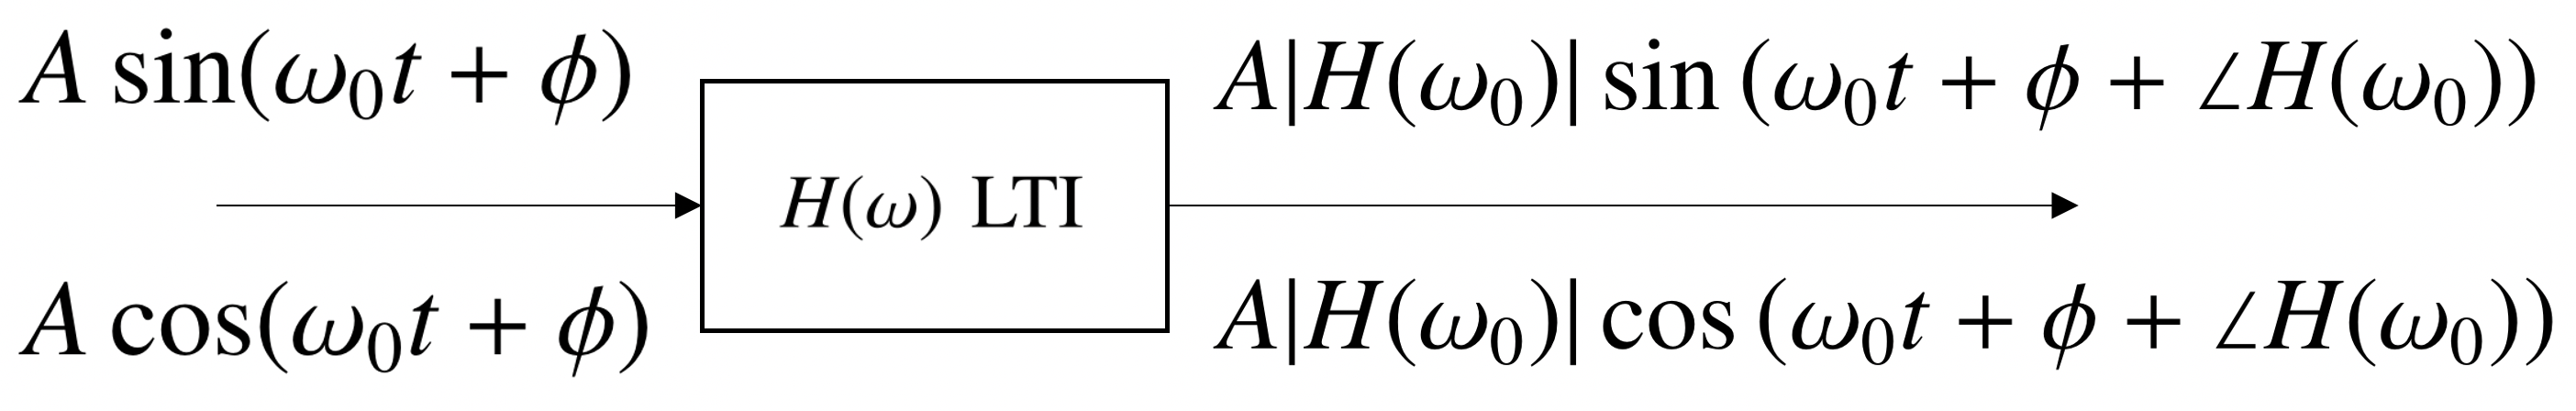
\includegraphics[width=\columnwidth]{figure.png}
\end{figure}
\end{document}
